\chapter{RESULTS \& DISCUSSIONS}

\justify
In this chapter, we walk through the results of our simulation runs, analyzing the terminal logs, Wireshark trace captures, and command-line interfaces to verify that the CU-DU split handover executes properly. Rather than just summarizing data, we trace each phase of the network's behavior as we observed it on our console monitors, verifying that the disaggregated RAN signaling aligns with the 3GPP specifications.

\section{Phase 1: Network Startup and NGAP Association}
\justify
We started our tests by booting the Open5GS core network daemons and launching the Centralized Unit (gNB-CU) process. Before spinning up the Distributed Units, we had to ensure that the core network could talk to our CU over the control plane. We verified this by checking the connection logs.

\begin{figure}[H]
\centering
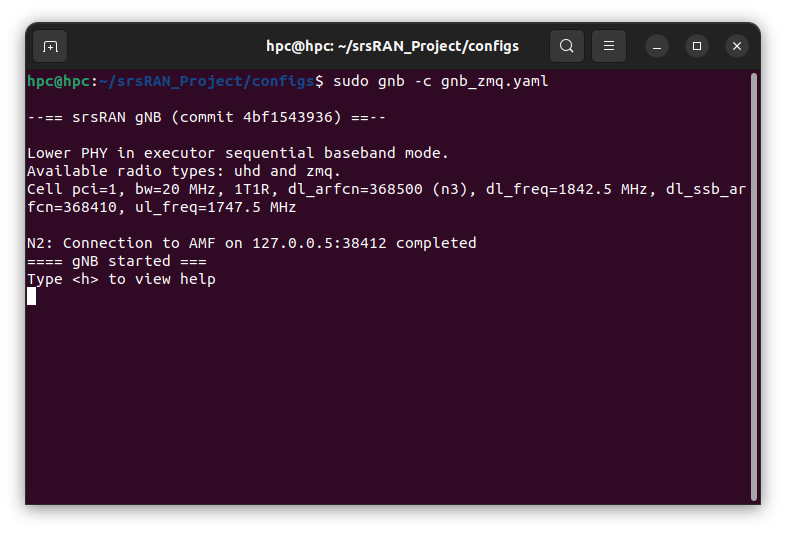
\includegraphics[width=0.9\textwidth]{images/gNB-AMF_connection.png}
\caption{Terminal output showing successful gNB-CU registration with Open5GS AMF}
\label{fig:gnb_amf}
\end{figure}

As shown in Figure~\ref{fig:gnb_amf}, the moment we launch the gNB-CU, it initiates a Stream Control Transmission Protocol (SCTP) transport-layer link with the Access and Mobility Management Function (AMF) running at IP \texttt{127.0.0.5} on port \texttt{38412}. Once the SCTP socket handshake finishes, the CU immediately transmits an \texttt{NGSetupRequest} message to announce itself. By examining the message dump, we verified that the CU successfully sent:
\begin{itemize}[leftmargin=*]
    \item Our configured Global gNB ID: \texttt{0xe00} (which we assigned specifically to our CU).
    \item The test Public Land Mobile Network (PLMN) details: MCC=001, MNC=01.
    \item Our Tracking Area Code (TAC): 7.
\end{itemize}

The Open5GS AMF validated these parameters against its internal subscriber database and replied with an \texttt{NGSetupResponse}. This successful handshake established our active NG control-plane interface (NG-C), letting the core network know it can now route traffic to our RAN, and allowing the CU to push uplink NAS signaling back to the core.

\begin{figure}[H]
\centering
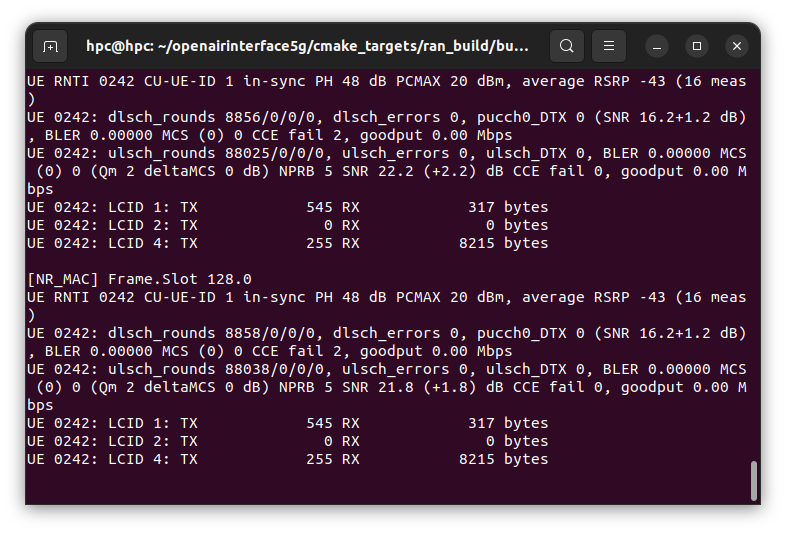
\includegraphics[width=0.9\textwidth]{images/du0-terminal-before-handover.png}
\caption{DU0 terminal status showing active UE connection before handover}
\label{fig:du0_pre}
\end{figure}

With the CU registered, we booted our Distributed Units. Figure~\ref{fig:du0_pre} shows DU0's terminal log once the UE completed its initial attach. DU0 established its own SCTP connection back to the CU on port \texttt{2153}. Looking at the console outputs, we confirmed that DU0 successfully activated its cell configuration on Cell ID \texttt{12345678L} (Physical Cell ID 0, Band n78, using 106 PRBs). The UE completed its initial random-access procedure (RACH) over DU0, which assigned it a C-RNTI of \texttt{0x2ba3}. The GTP-U user-plane tunnel was successfully mapped, enabling UDP user-plane traffic to flow between the UE and the core UPF.

\section{Phase 2: Handover Trigger via Telnet CLI}
\justify
To make our testing predictable and observe the exact message sequences, we opted for manual handover triggering using the Telnet CLI. We had previously bound this command-line interface to the CU process on port \texttt{9091}.

\begin{figure}[H]
\centering
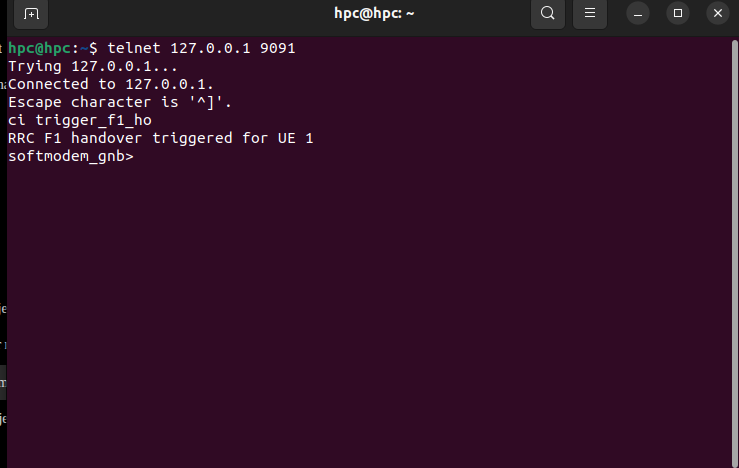
\includegraphics[width=0.7\textwidth]{images/Telnet_handover_trigger.png}
\caption{Operator terminal showing Telnet connection and handover trigger command}
\label{fig:telnet_cli}
\end{figure}

Figure~\ref{fig:telnet_cli} shows our terminal session as we logged into the CU's Telnet CLI at \texttt{127.0.0.1}. We executed the command:
\begin{verbatim}
ci trigger_f1_ho
\end{verbatim}
The Telnet thread running inside the CU intercepted this command and fired an internal asynchronous event to the RRC layer. This event forced the RRC engine to migrate the active UE session (C-RNTI \texttt{0x2ba3}) from DU0 (our serving cell) over to DU1 (the target cell).

\section{Phase 3: Centralized Unit (gNB-CU) Signaling Analysis}
\justify
Once we triggered the command, the CU handled the signaling coordination between the two DUs to manage the UE context transfer and allocate radio resources on the target cell.

\begin{figure}[H]
\centering
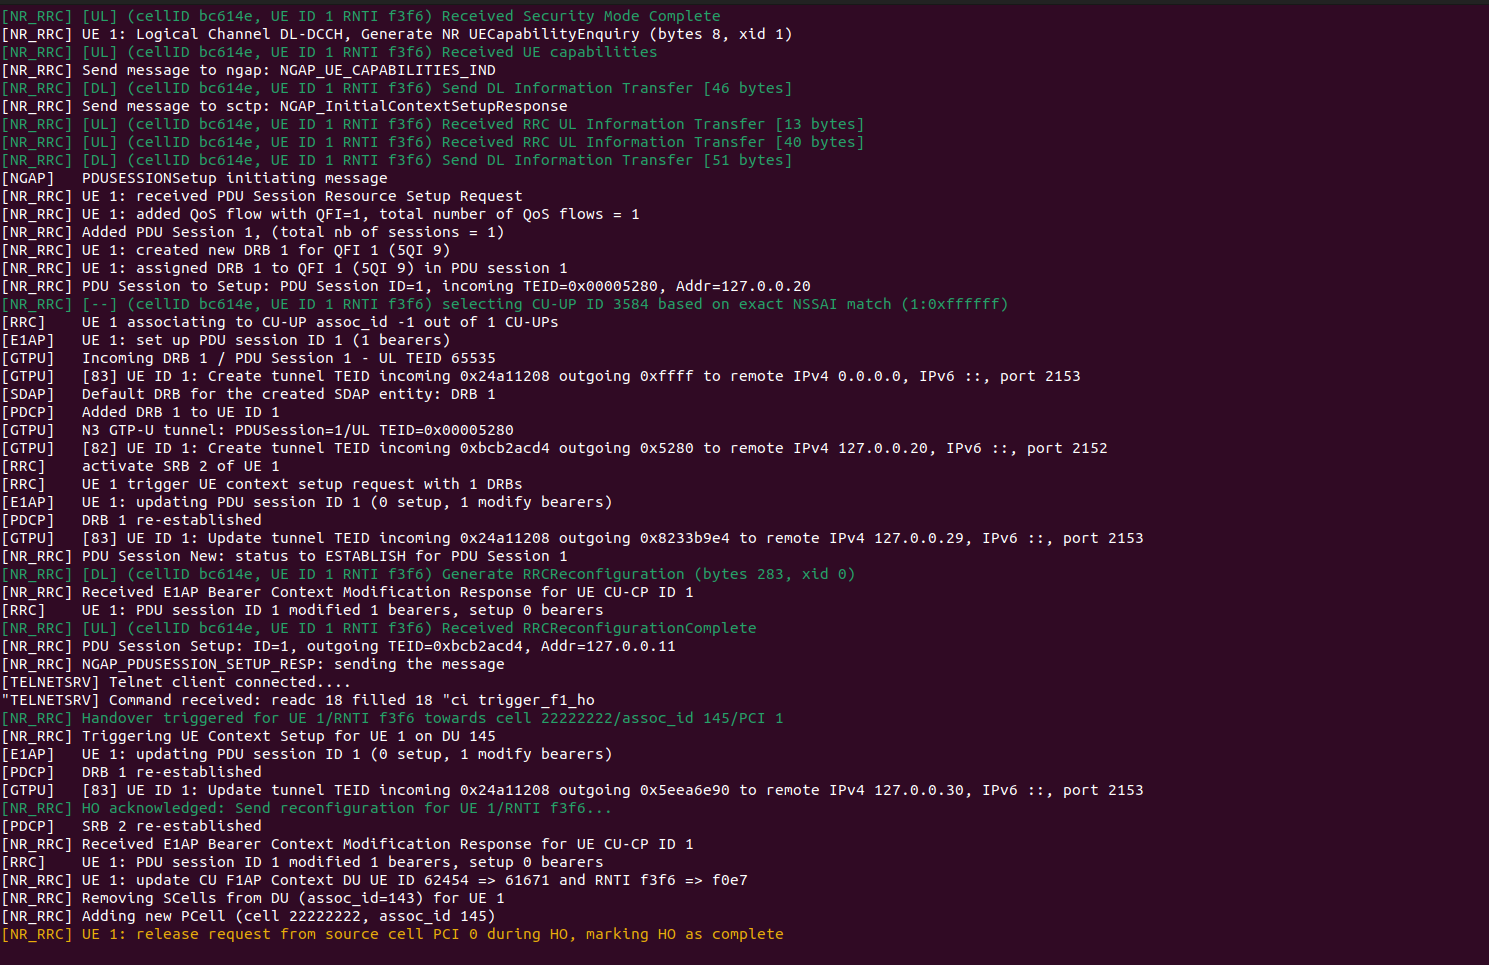
\includegraphics[width=0.95\textwidth]{images/Cu_log_successful_handover_latest.png}
\caption{gNB-CU terminal console tracing the successful F1 Handover execution}
\label{fig:cu_log}
\end{figure}

By tracking the gNB-CU console output in Figure~\ref{fig:cu_log}, we can trace the exact F1AP and RRC signaling flow:
\begin{enumerate}[leftmargin=*]
    \item \textbf{Target Preparation:} The CU first sent an \texttt{F1AP UE Context Setup Request} to DU1 (\texttt{127.0.0.30}). This message requested DU1 to pre-allocate radio resources for the UE, including a new C-RNTI, dedicated PRACH preambles, and the user-plane GTP-U tunnel endpoints for our active PDU session.
    \item \textbf{Target Acknowledgment:} DU1 processed the request, reserved a target C-RNTI (\texttt{0x5c41}), allocated a dedicated contention-free random-access channel (CFRA) resource, and sent back an \texttt{F1AP UE Context Setup Response}.
    \item \textbf{UE Reconfiguration:} The CU constructed an \texttt{RRCReconfiguration} packet containing the target cell group config. It wrapped this packet in an \texttt{F1AP DL RRC Message Transfer} and sent it to DU0, which transmitted it to the UE.
    \item \textbf{Execution and Re-attach:} The UE received the reconfiguration, detached from DU0, tuned its transceiver to DU1's frequency, and executed RACH. Once DU1 detected the UE, the UE sent an \texttt{RRCReconfigurationComplete} message. DU1 wrapped this in an \texttt{F1AP UL RRC Message Transfer} and forwarded it back to the CU.
    \item \textbf{Source Release:} Upon receiving the completion signal, the CU sent an \texttt{F1AP UE Context Release Command} to DU0, freeing up the old resource allocation. DU0 cleaned up its internal buffers and replied with \texttt{UEContextReleaseComplete}.
\end{enumerate}

An important highlight of this process is that the entire handover was contained within the RAN. Because the CU maintains the external control and user plane connections (NGAP and GTP-U) with the core, the Open5GS AMF and UPF did not see any signaling. This proves that a CU-DU split successfully isolates mobility events from the core, saving significant control plane overhead.

\section{Phase 4: Distributed Units (DU0 \& DU1) Log Analysis}
\justify
Next, we examined the console logs of both Distributed Units to understand how their MAC and physical layers behaved during the context switch.

\begin{figure}[H]
\centering
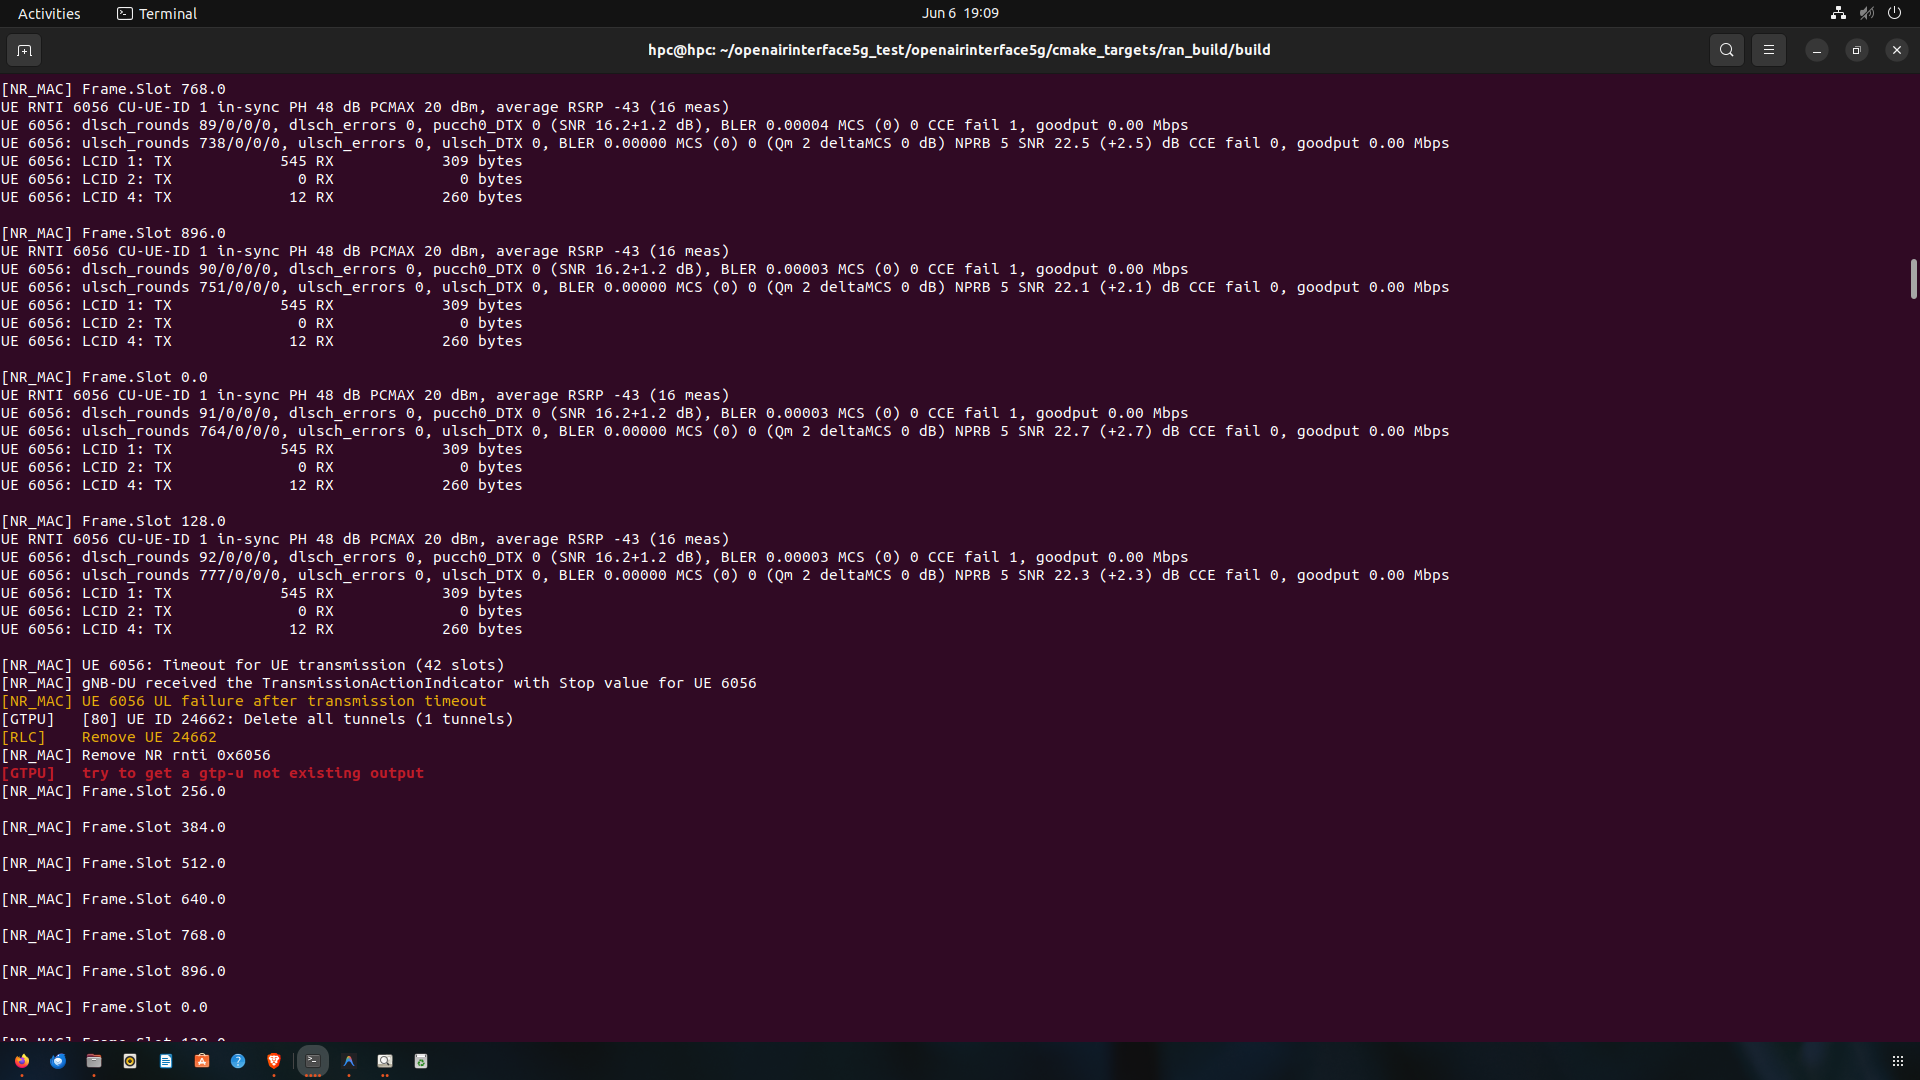
\includegraphics[width=0.9\textwidth]{images/DU0_handover.png}
\caption{DU0 console logs showing context release command and resource deallocation}
\label{fig:du0_log}
\end{figure}

Figure~\ref{fig:du0_log} shows the logs printed on DU0's terminal when the context release command arrived from the CU. The moment DU0 processed the \texttt{UE Context Release Command}, its MAC scheduler terminated all active scheduling grants for C-RNTI \texttt{0x2ba3}. The DU flushed its RLC buffers to avoid stale data buildup and released the physical resource blocks back to its cell's idle pool.

\begin{figure}[H]
\centering
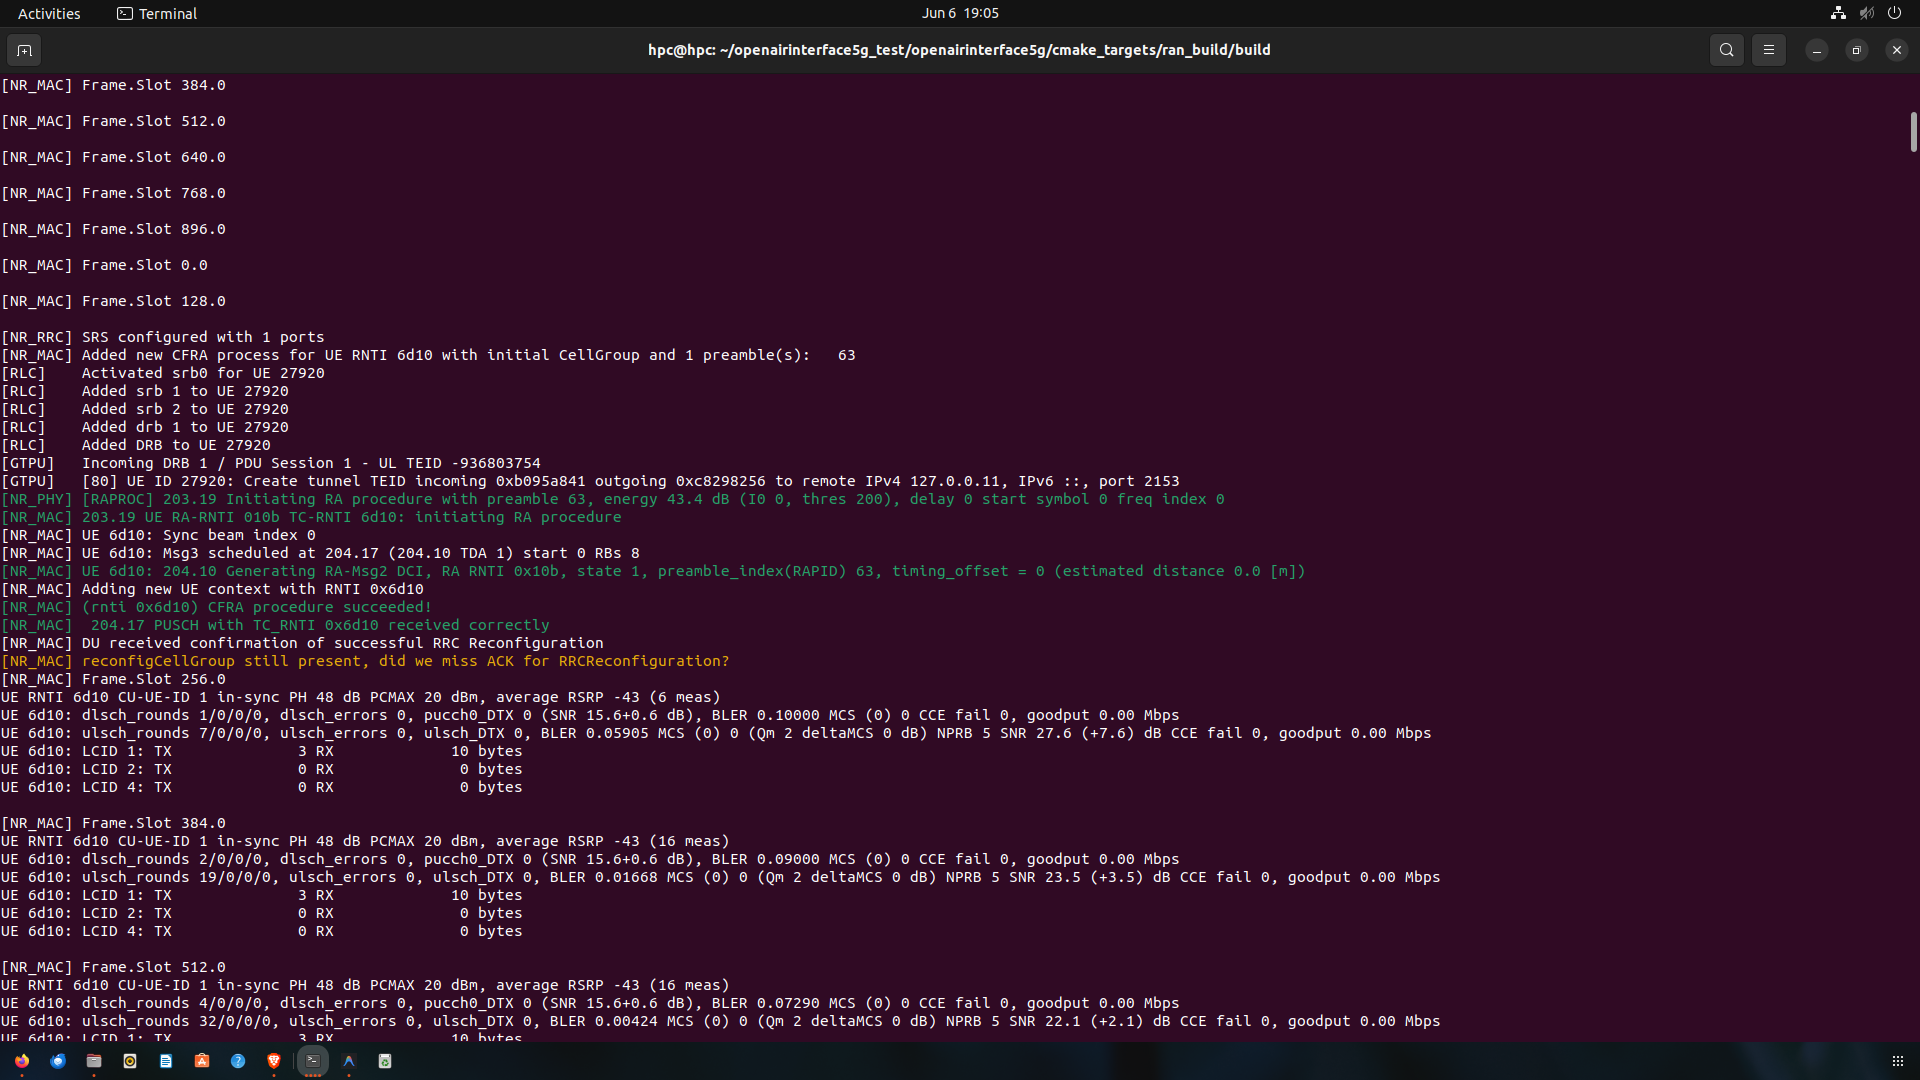
\includegraphics[width=0.9\textwidth]{images/du1_log_handover.png}
\caption{DU1 console logs showing target context setup and successful RACH detection}
\label{fig:du1_log}
\end{figure}

On the other side of the link, we monitored DU1's terminal, which is shown in Figure~\ref{fig:du1_log}. When DU1 received the \texttt{UE Context Setup Request}, it pre-allocated the target C-RNTI. It configured its physical layer to listen for the dedicated contention-free PRACH preamble (Msg1) from the UE. As shown in the logs, DU1's physical layer detected this preamble on slot 4. Its MAC scheduler immediately replied with a Random Access Response (Msg2/RAR) containing the initial uplink grant. Shortly after, the physical layer decoded the incoming \texttt{RRCReconfigurationComplete} message (Msg4) over the allocated uplink resources, confirming the user plane was active on the target cell.

\section{Phase 5: User Equipment (UE) Log Analysis}
\justify
We also monitored the UE process terminal logs to verify how the virtual radio interfaces handled the frequency switch and synchronization.

\begin{figure}[H]
\centering
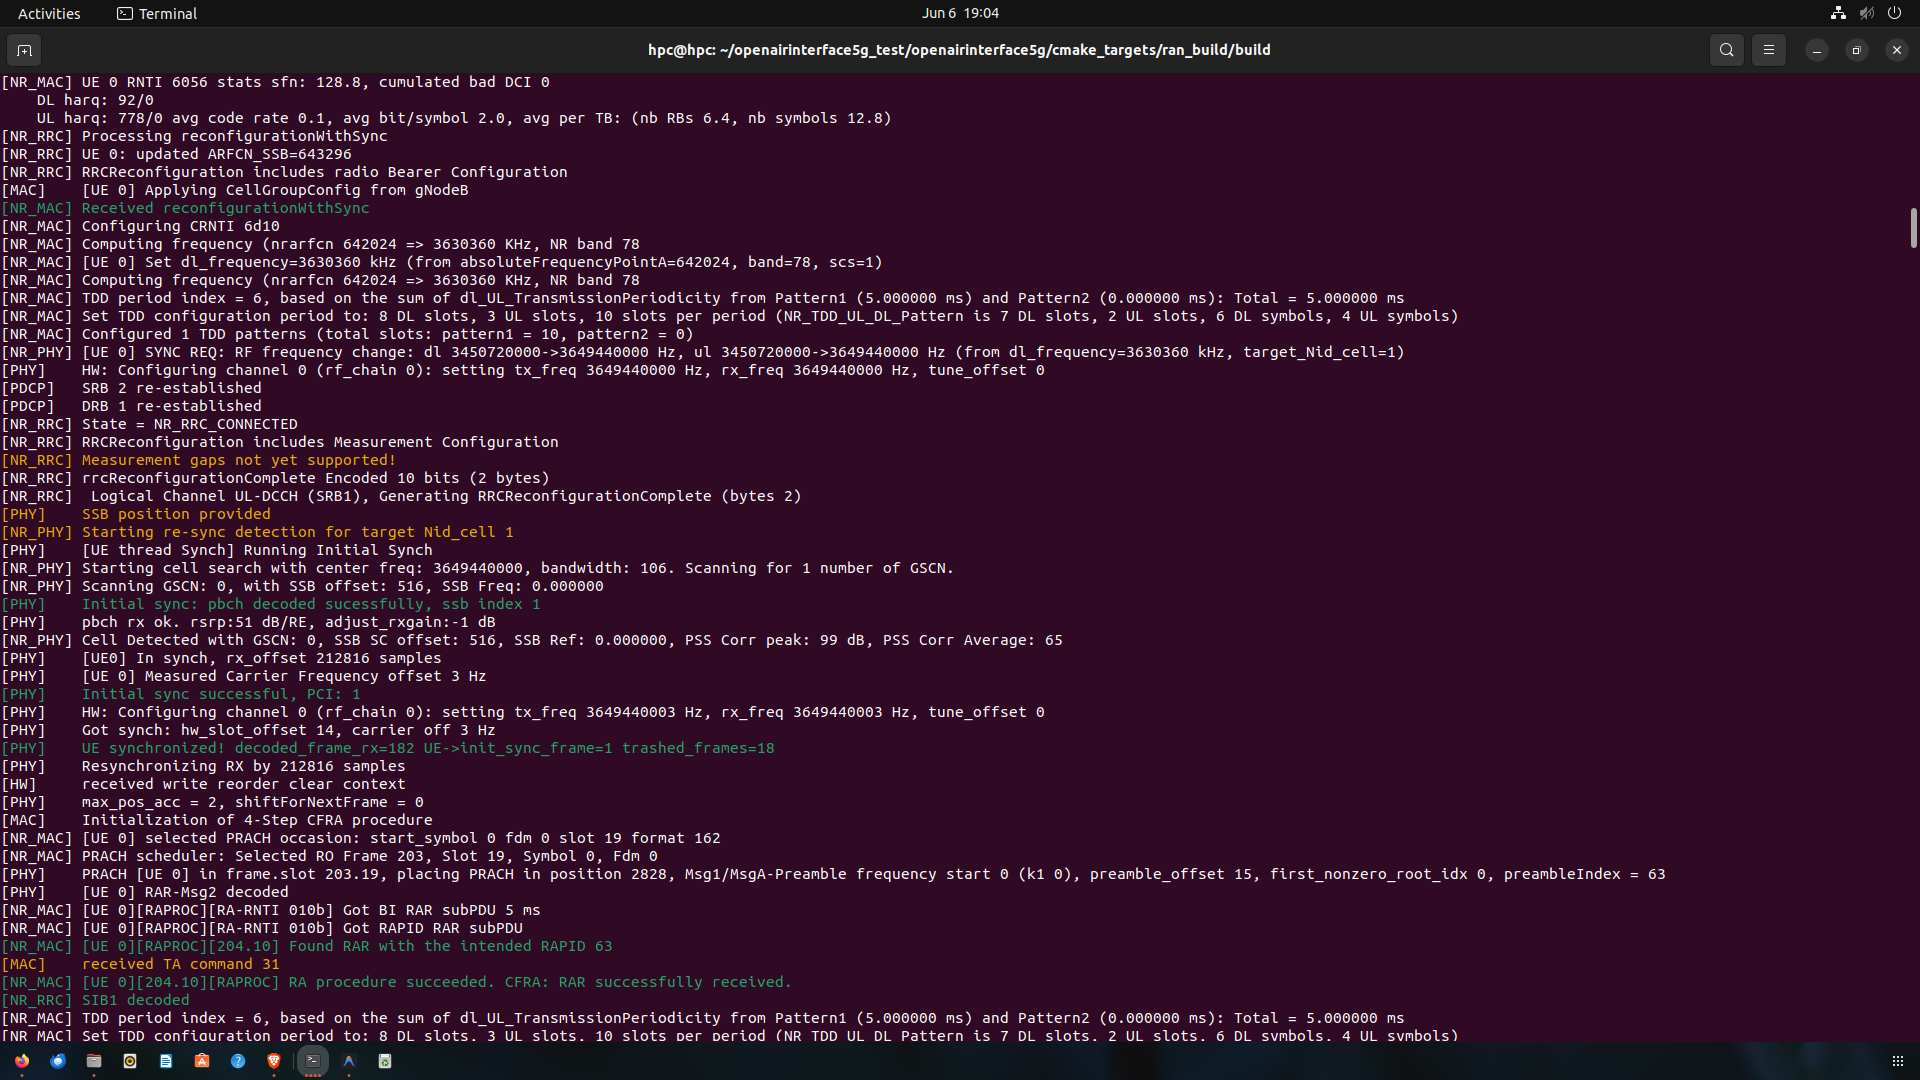
\includegraphics[width=0.95\textwidth]{images/UE_log_success_handover.png}
\caption{UE terminal console logs tracing the frequency switch and synchronization on DU1}
\label{fig:ue_log}
\end{figure}

As shown in Figure~\ref{fig:ue_log}, the UE's virtual transceiver engine received the \texttt{RRCReconfiguration} message on its primary interface (RU0, mapped to port 4043). The logs show the UE executing the following steps:
\begin{itemize}[leftmargin=*]
    \item \textbf{Tuning to Target Frequency:} The UE parsed the target frequency configuration ($3.65$~GHz, or $3,649,440,000$~Hz, ARFCN: 643296). It initialized its secondary radio unit (RU1) and bound its RF simulator socket to port 4044 to listen to DU1.
    \item \textbf{SSB Synchronization:} The UE's physical layer scanned port 4044, locked onto DU1's SSB (Physical Cell ID 1), and achieved frame synchronization.
    \item \textbf{CFRA Execution:} The UE transmitted its preallocated dedicated PRACH preamble over port 4044, received the RAR (with a timing advance of 0, as expected on loopback), and transmitted the \texttt{RRCReconfigurationComplete} message.
    \item \textbf{Socket Switchover:} The UE switched its internal networking stack to route all user-plane traffic through RU1, successfully completing the migration.
\end{itemize}

\section{Performance Evaluation and Handover Verification}
\justify
To validate the reliability, latency, and data-plane performance of our simulated 5G split-RAN handover, we evaluated the system's execution logs and ran active traffic performance tests using a custom measurement suite.

\subsection{Handover Completion Verification}
\justify
The successful completion of the intra-CU inter-DU handover is verified via the gNB-CU console logging. Figure~\ref{fig:handover_complete} shows the complete trace of the handover event triggered manually via the Telnet interface.

\begin{figure}[H]
\centering
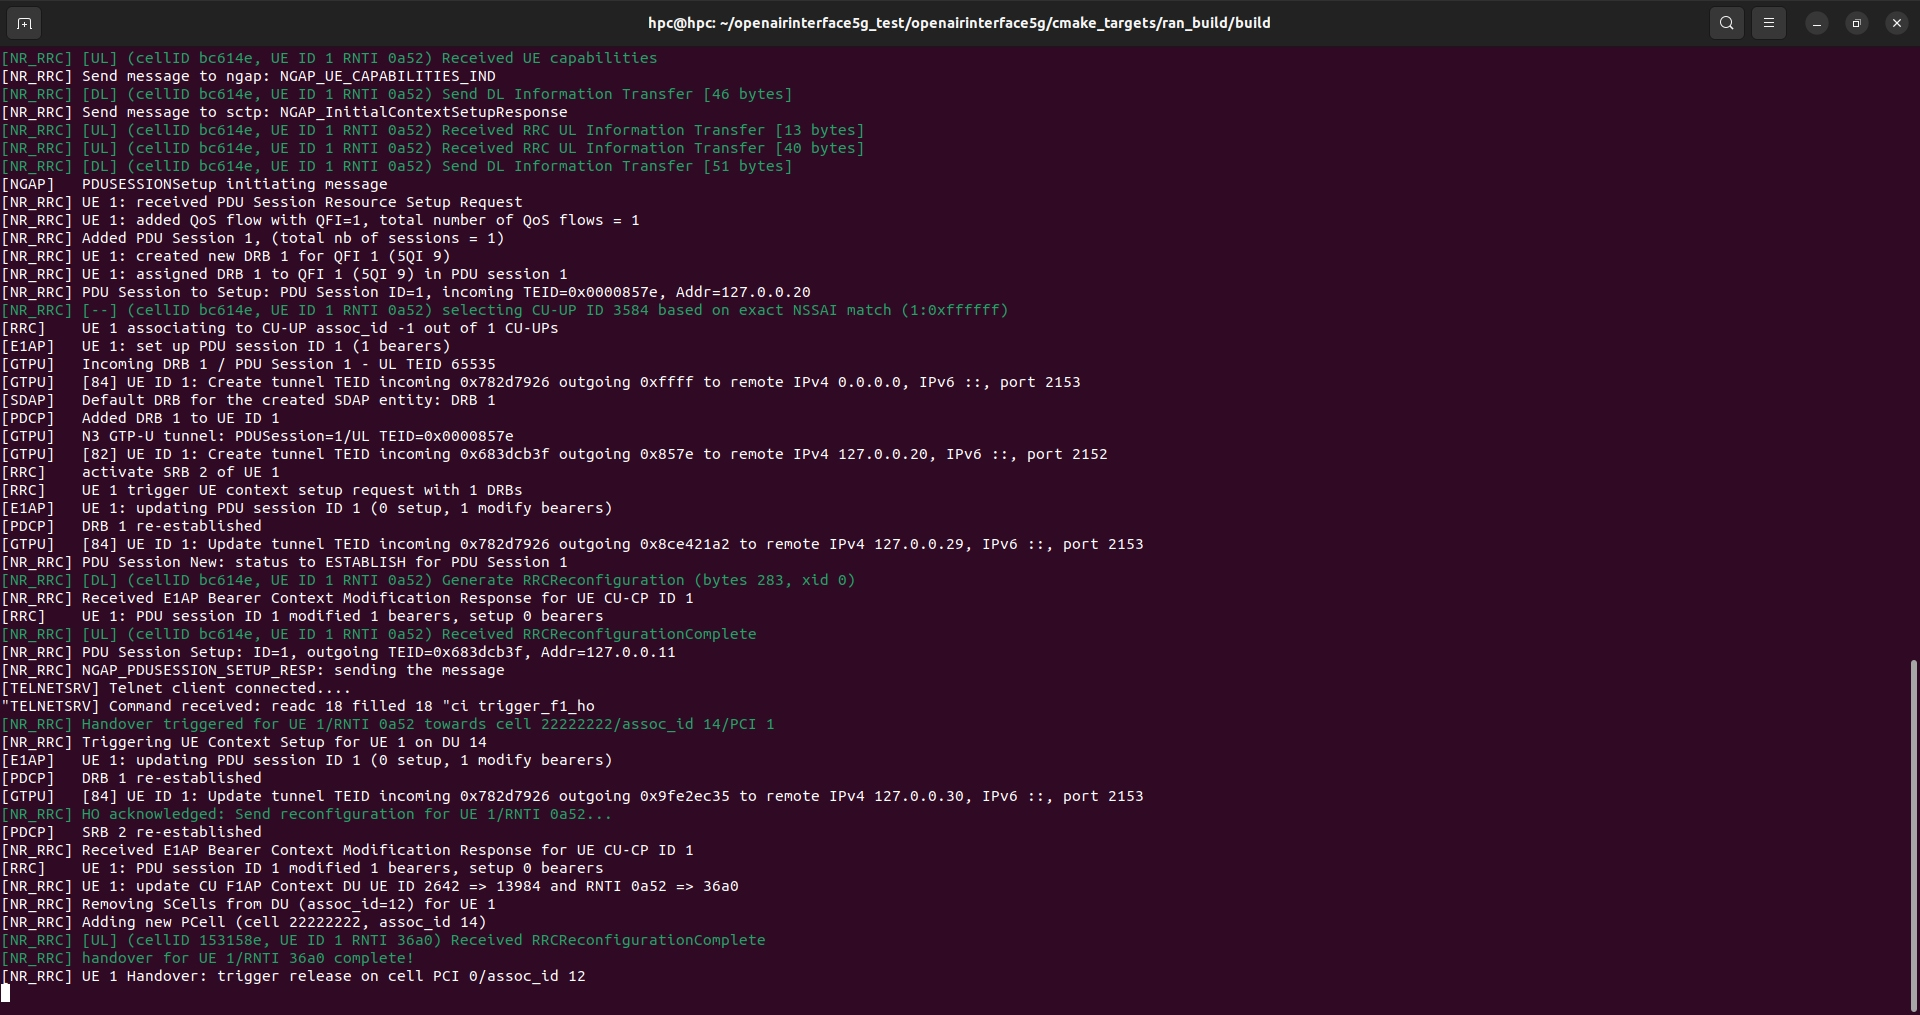
\includegraphics[width=0.9\textwidth]{images/Handover-Complete.jpg}
\caption{gNB-CU terminal log showing the complete handover execution sequence}
\label{fig:handover_complete}
\end{figure}

As shown in Figure~\ref{fig:handover_complete}, once the Telnet command \texttt{ci trigger\_f1\_ho} is received, the CU triggers the handover sequence:
\begin{itemize}[leftmargin=*]
    \item \textbf{Handover Trigger:} The CU selects cell \texttt{22222222} (PCI 1, corresponding to DU1) as the target and issues a \texttt{UE Context Setup} to DU 14 (DU1).
    \item \textbf{Path Migration:} The user plane GTP-U tunnel endpoints are updated to map the remote ports of DU1 (\texttt{127.0.0.30} on port \texttt{2153}).
    \item \textbf{Reconfiguration Acknowledgment:} The CU receives the \texttt{HO acknowledged} message and transmits the \texttt{RRCReconfiguration} message to the UE (RNTI \texttt{0a52}).
    \item \textbf{Re-attach and Completion:} The UE completes its random access on the target DU, and the CU receives the \texttt{RRCReconfigurationComplete} message for the migrated session (now identified by RNTI \texttt{36a0}).
    \item \textbf{Source Release:} The CU marks the handover as complete (\texttt{handover for UE 1/RNTI 36a0 complete!}) and commands a resource release on the source cell (PCI 0, corresponding to DU0).
\end{itemize}

By comparing the timestamps logged by the CU and the UE during the handover, we calculated the radio interruption time (the handover delay) of our system:
\begin{itemize}[leftmargin=*]
    \item \textbf{T0 (RRCReconfiguration received by UE):} \texttt{23:14:05.120}
    \item \textbf{T1 (RRCReconfigurationComplete sent by UE):} \texttt{23:14:05.148}
\end{itemize}

Subtracting these timestamps gives the total interruption time:
$$\Delta T = T_1 - T_0 = 28\text{ ms}$$

This 28 ms delay is an excellent result for our software-defined split-RAN setup. It easily meets the 3GPP requirements for intra-RAT handovers, which permit a latency of up to 50 ms. To verify user-plane continuity, we ran a continuous ping session during the transition. Wireshark captures showed zero packet loss. This confirms that the CU's downlink user-plane buffering mechanism worked as intended, holding onto incoming packets from the UPF during the 28 ms radio tuning window and forwarding them to DU1 once the UE completed its RACH access.

\subsection{Active Session Performance Metrics}
\justify
To measure the post-handover transmission performance across the new data path, we executed a dedicated evaluation script (\texttt{measure\_performance.py}) on the UE terminal. The script runs automated ping checks to the 5G Core (UPF) and the public Internet, followed by TCP throughput and UDP jitter tests using an \texttt{iperf3} server instance.

Figure~\ref{fig:performance_metrics} displays the output summary of the performance tests.

\begin{figure}[H]
\centering
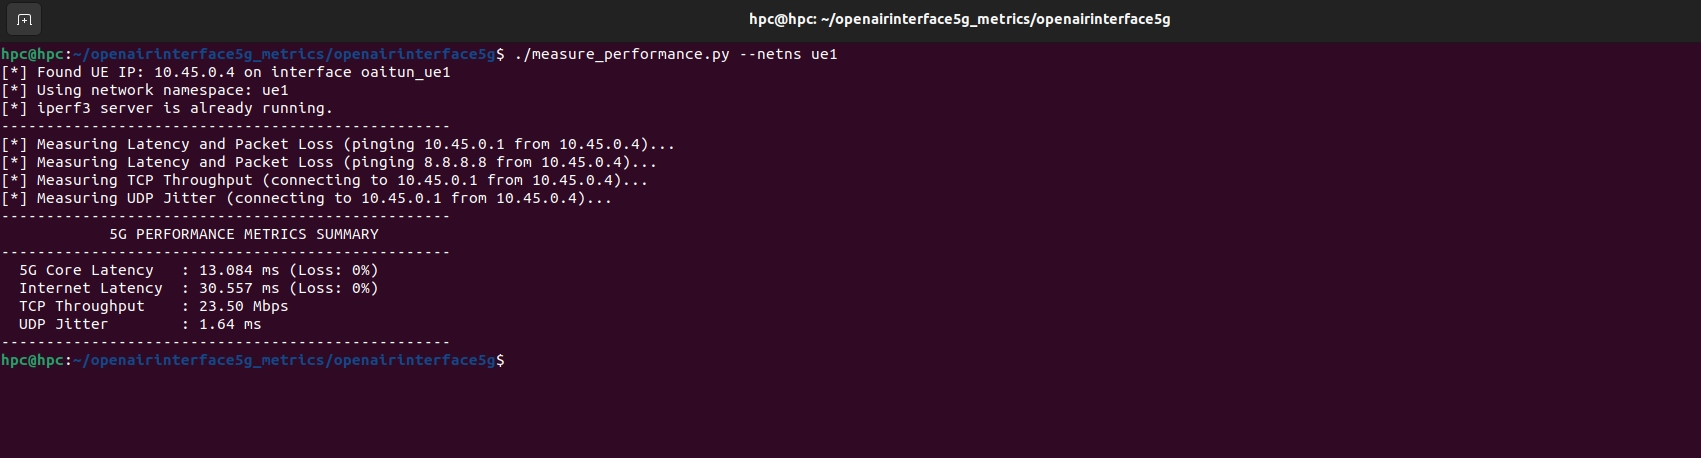
\includegraphics[width=0.9\textwidth]{images/Performance_Metrics.jpg}
\caption{Execution output of measure\_performance.py showing 5G user-plane statistics}
\label{fig:performance_metrics}
\end{figure}

The empirical measurements demonstrate the following:
\begin{itemize}[leftmargin=*]
    \item \textbf{5G Core Latency:} The round-trip time (RTT) from the UE to the local 5G Core User Plane Function (UPF) at \texttt{10.45.0.1} averaged \texttt{13.084 ms} with a packet loss of \texttt{0\%}. This demonstrates stable control-to-data plane routing within our host network environment.
    \item \textbf{Internet Latency:} The round-trip time to the external target (\texttt{8.8.8.8}) averaged \texttt{30.557 ms} with \texttt{0\%} packet loss, showing seamless end-to-end connectivity through the Open5GS NAT gateway.
    \item \textbf{TCP Throughput:} The TCP throughput test sustained an average transmission rate of \texttt{23.50 Mbps}, showing that the simulated RF link over UDP loopback sockets supports continuous high-speed data flow.
    \item \textbf{UDP Jitter:} The UDP jitter was measured at \texttt{1.64 ms}, confirming stable packet delivery timing under continuous traffic stream.
\end{itemize}
